\subsection{Ablation study for GCF}
Meng Liu et. al does not present an ablation study for BiTGCF and GCF, which LightGCN showed is important with their to the ablation study conducted on NGCF \cite{lightgcn,BiTGCF}.
In this section we conduct an ablation study on GCF to get an understanding of the effect that the different parts of embedding propagation and layer combination have.
Examples of the equations can be seen on \autoref{eq:GCF-minus-sc}, \autoref{eq:GCF-only-IP} and \autoref{eq:GCF-minus-IP}.
\textit{GCF-minus-sc} can be seen on \autoref{eq:GCF-minus-sc} where the self-connection has been removed.
On \autoref{eq:GCF-only-IP} only the inner product of the neighbor remains, and is called \textit{GCF-only-IP}
\autoref{eq:GCF-minus-IP} the inner product has been removed and is called \textit{GCF-minus-IP}.
There are also examples where GCF utilizes weighted summation as layer combination as used in LightGCN.
Weighted summation can be seen on \autoref{eq:lightgcn-sum}.
These are named \textit{GCF-sum}.
When LightGCN is tested with concatenation as layer combination it is called \textit{LightGCN-concat}.
\begin{equation}
    \mathbf{e}_{u}^{(k+1)} = \sum^{}_{i \in \mathcal{N}_u}  \frac{1}{\sqrt{|\mathcal{N}_u||\mathcal{N}_i|}}\left( \mathbf{e}_i^{(k)} + \mathbf{e}_i^{(k)} \odot \mathbf{e}_u^{(k)} \right)
    \label{eq:GCF-minus-sc}
\end{equation}
\begin{equation}
    \mathbf{e}_{u}^{(k+1)} = \mathbf{e}_{u}^{(k)} + \sum^{}_{i \in \mathcal{N}_u}  \frac{1}{\sqrt{|\mathcal{N}_u||\mathcal{N}_i|}} \mathbf{e}_i^{(k)} \odot \mathbf{e}_u^{(k)}
    \label{eq:GCF-only-IP}
\end{equation}
\begin{equation}
    \mathbf{e}_{u}^{(k+1)} = \mathbf{e}_{u}^{(k)} + \sum^{}_{i \in \mathcal{N}_u}  \frac{1}{\sqrt{|\mathcal{N}_u||\mathcal{N}_i|}} \mathbf{e}_i^{(k)}
    \label{eq:GCF-minus-IP}
\end{equation}
\autoref{fig:GCF-NDCG-ablation-study} and \autoref{fig:GCF-recall-ablation-study} contains the GCF ablation study, where all GCF modifications still have the inner product between users and items, except for LightGCN.
The x-axis describes the every time the epochs increases by 20, and the y-axis is how well it performs regarding to NDCG or Recall.
The methods are as described here:\\
\begin{itemize}
    \item \textbf{GCF}: The original GCF method as described in \autoref{subsubsec:GCF-embed-propagation}.
    \item \textbf{GCF-minus-sc}: GCF without self connections
    \item \textbf{GCF-only-IP}:  GCF where $e_i^{(k)}$ has been removed in \autoref{eq:GCF-embedding}, so that GCF's graph convolutions only considers the inner product of users and items.
    \item \textbf{GCF-only-IP-minus-sc}: Implemented as GCF-only-ip but without self connections.
    \item \textbf{GCF-minus-IP}: GCF where inner product has been removed.
    \item \textbf{GCF-minus-IP-and-sc}: Same as GCF-minus-IP, but without self connections.
    \item \textbf{LightGCN-concat}: LightGCN with concatenation as layer combination.
    \item \textbf{LightGCN}: Original LightGCN as described in \autoref{subsubsec:LightGCN-embed-propagation}.
    \item \textbf{LightGCN-plus-sc}: LightGCN, but with self connections.
    \item \textbf{GCF-sum-only-IP}: Implemented as GCF-only-IP except that the layer combination method used is weighted summation.
    \item \textbf{GCF-sum}: GCF where the layer combination has been changed to weighted summation instead of concatenation.
    \item \textbf{GCF-sum-minus-sc}: Implemented as GCF-sum but without self connections.
\end{itemize}
\begin{figure}[h!]
    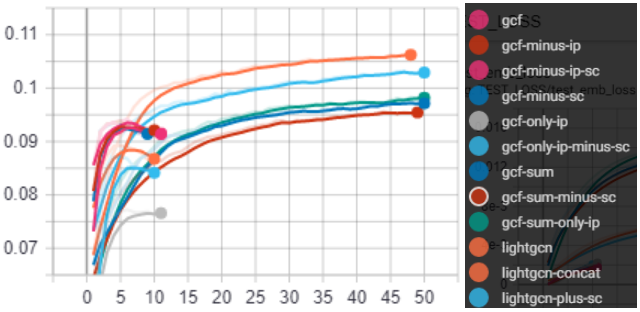
\includegraphics[width=\linewidth]{figures/gcf-all-ndcg.png}
    \caption{NDCG@50 for the Yelp2020 dataset.}
    \label{fig:GCF-NDCG-ablation-study}
\end{figure}
\begin{figure}[h!]
    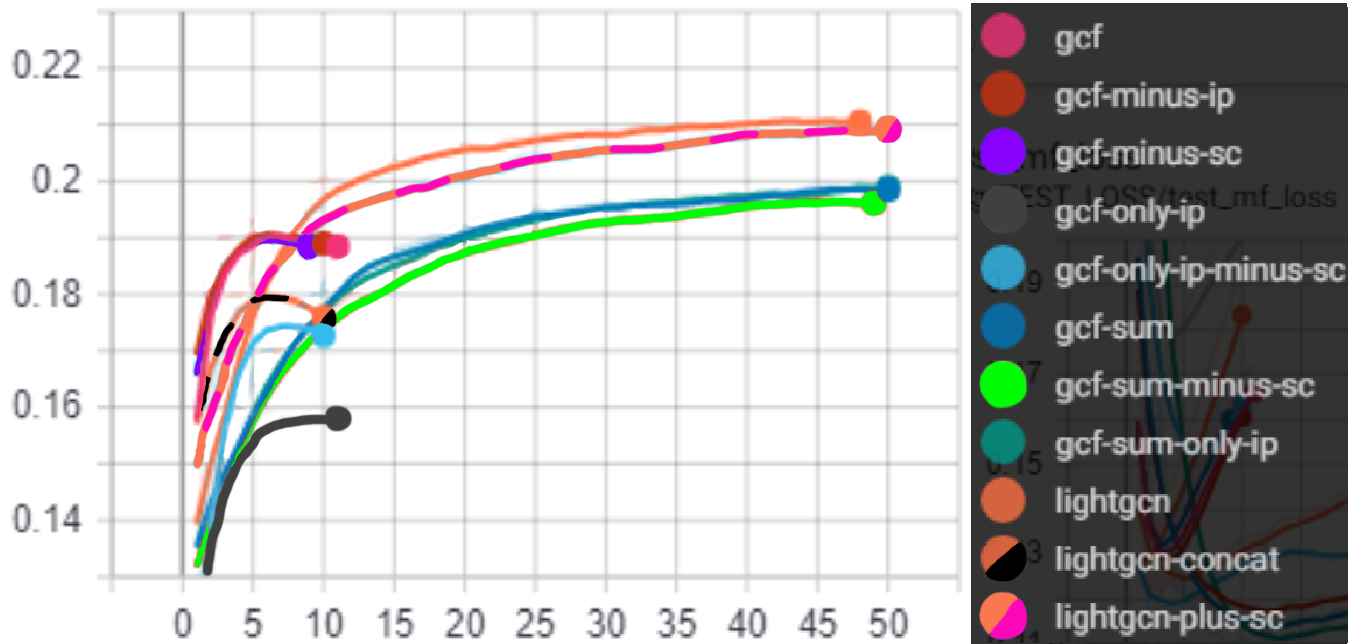
\includegraphics[width=\linewidth]{figures/gcf-all-recall.png}
    \caption{Recall@50 on the Yelp2020 dataset.}
    \label{fig:GCF-recall-ablation-study}
\end{figure}
From \autoref{fig:GCF-NDCG-ablation-study} and \autoref{fig:GCF-recall-ablation-study} it can be seen that the methods that do utilize concatenation as layer combination generally perform worse than the methods that utilize weigthed summation.
The results can also be seen on \autoref{tab:ablation-results}
It is also noticeable that most concatenation methods learn faster than the summation methods.
These experiments all have the dropout ratio set to 0, so it could be because the concatenation methods start overfitting.
This is likely because weighted summation is more sensitive to changes in the embeddings, and using both neighboring convolutions and inner product can create contradictions.
\begin{table}[]
    \centering
    \begin{tabular}{|l|l|l|}
        \hline
                             & NDCG    & Recall \\ \hline
        GCF                  & 0.09092 & 0.1869 \\ \hline
        GCF-minus-ip         & 0.09179 & 0.1881 \\ \hline
        GCF-minus-ip-sc      & 0.09087 & 0.1871 \\ \hline
        GCF-minus-sc         & 0.09084 & 0.1879 \\ \hline
        GCF-only-ip          & 0.07659 & 0.1587 \\ \hline
        GCF-only-ip-minus-sc & 0.08338 & 0.1712 \\ \hline
        LightGCN-concat      & 0.0856  & 0.1735 \\ \hline
        LightGCN             & 0.1064  & 0.2106 \\ \hline
        GCF-sum              & 0.09724 & 0.1988 \\ \hline
        GCF-sum-minus-sc     & 0.0956  & 0.1962 \\ \hline
        GCF-sum-only-ip      & 0.09843 & 0.199  \\ \hline
        LightGCN-plus-sc     & 0.1031  & 0.2098 \\ \hline
    \end{tabular}
    \caption{NDCG and Recall of the changed methods.}
    \label{tab:ablation-results}
\end{table}
\begin{figure}[h!]
    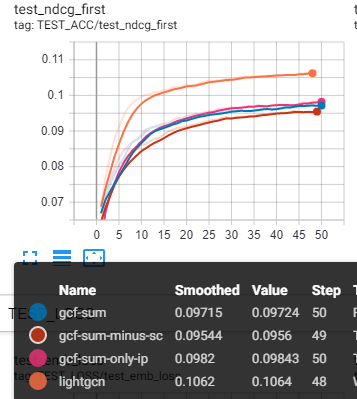
\includegraphics[width=\linewidth]{figures/gcf-sum-ndcg.png}
    \caption{NDCG@50 for the compared methods that utilize summation as layer combination on the Yelp2020 dataset.}
    \label{fig:GCF-sum-NDCG-ablation-study}
\end{figure}
\begin{figure}[h!]
    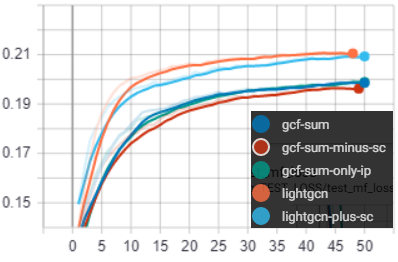
\includegraphics[width=\linewidth]{figures/gcf-sum-recall.png}
    \caption{Recall@50 on the compared methods that utilize summation as layer combination on the Yelp2020 dataset.}
    \label{fig:GCF-sum-recall-ablation-study}
\end{figure}
Looking at \autoref{fig:GCF-sum-NDCG-ablation-study} and \autoref{fig:GCF-sum-recall-ablation-study} it can be seen that LightGCN performs better than the other GCF methods that utilize weighted summation as layer combination.
\begin{figure}[h!]
    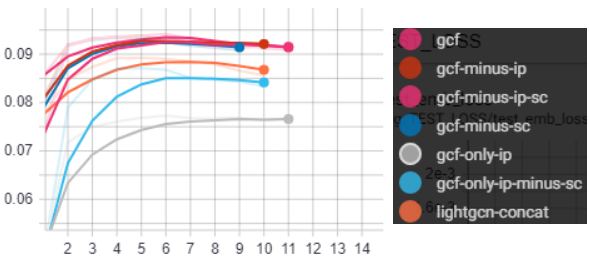
\includegraphics[width=\linewidth]{figures/gcf-ndcg-concat.png}
    \caption{NDCG@50 for the compared methods that utilize concatenation as layer combination on the Yelp2020 dataset.}
    \label{fig:GCF-NDCG-concat-ablation-study}
\end{figure}
\begin{figure}[h!]
    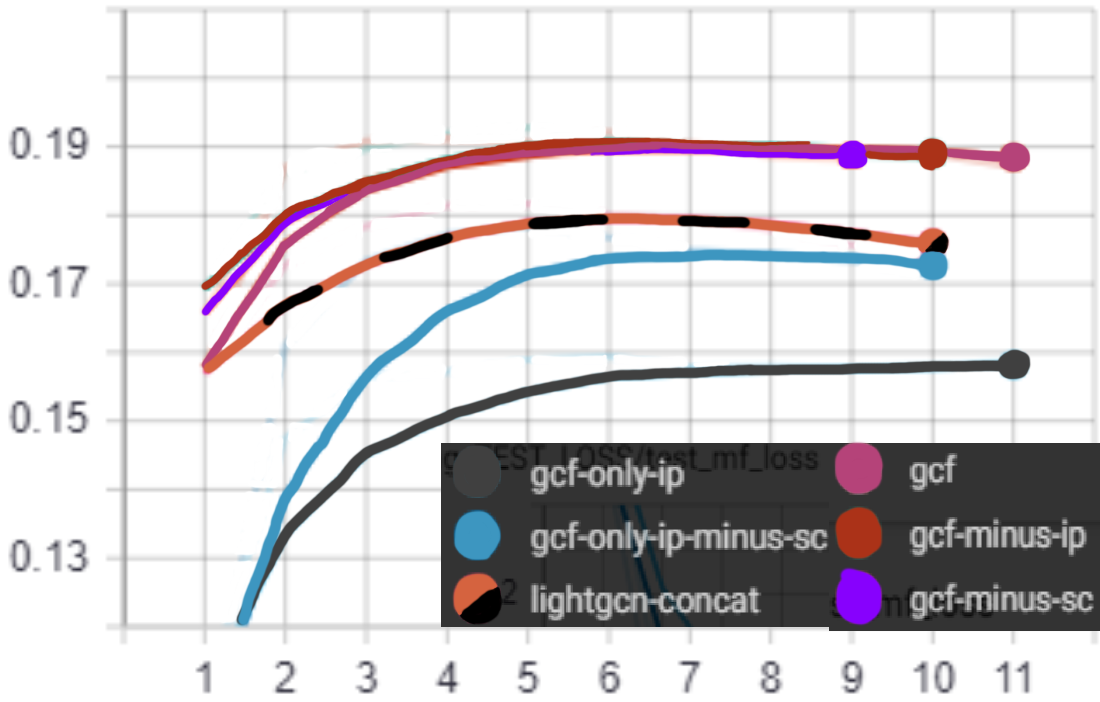
\includegraphics[width=\linewidth]{figures/gcf-concat-recall.png}
    \caption{Recall@50 for the compared methods that utilize concatenation as layer combination on the Yelp2020 dataset.}
    \label{fig:GCF-recall-concat-ablation-study}
\end{figure}
On \autoref{fig:GCF-NDCG-concat-ablation-study} and \autoref{fig:GCF-recall-concat-ablation-study} GCF without self connections performs a small amount better than GCF.
Only keeping inner product makes them perform worse when using concatenation as layer combination.
Interestingly \textit{gcf-only-ip-minus-sc} performs better than \textit{gcf-only-ip}, which can indicate that self connections are harmful for performance, if you only use inner product in the convolutions.
